\documentclass[11pt,letterpaper]{article}
\usepackage[T1]{fontenc}
\usepackage{lmodern,amsmath,amssymb,booktabs,longtable,graphicx}
\usepackage[margin=1in]{geometry}
\usepackage[hidelinks]{hyperref}
\newtheorem{theorem}{Theorem}
\newtheorem{proposition}[theorem]{Proposition}
\newtheorem{lemma}[theorem]{Lemma}
\newtheorem{corollary}[theorem]{Corollary}
\newtheorem{remark}[theorem]{Remark}
\renewcommand{\square}{\vcenter{\hbox{\rule{.72ex}{.72ex}}}}
\newenvironment{proof}{\par\smallskip\noindent\textit{Proof.}\ }{\nobreak\hfill\rule{.72ex}{.72ex}\par\smallskip}
\newcommand{\Z}{\mathbb Z}
\newcommand{\N}{\mathbb N}
\newcommand{\authorline}{Iaroslav Argunov}
\newcommand{\paperhead}[1]{\title{#1}\author{\authorline}\date{18 November 2026}\maketitle}
\renewcommand{\arraystretch}{1.12}
\setlength{\parindent}{1.1em}
\raggedbottom

\hypersetup{pdfauthor={Iaroslav Argunov},pdftitle={Symmetric open meanders with two marked ends}}
\begin{document}
\paperhead{Symmetric open meanders with two marked ends}
\begin{abstract}
Let \(K_k\) be the number of centrally symmetric open meander shapes with \(2k+1\) crossings in the convention of Legendre. We compute \(K_k\) through \(k=45\), recovering all entries through \(k=32\) in the public data of Hogan. We keep the boundary path attached to one marked end and join each pair of endpoints as soon as every completion requires it. For a fixed deficit \(j\) of the crossing height we give a cyclotomic denominator and prove that the resulting count is eventually a quasipolynomial of degree \(2j\). Its period divides \(\operatorname{lcm}(1,3,\ldots,2j+1)\). Legendre's orbit formula then gives the total number of open shapes at every odd crossing count through 75.
\end{abstract}

\section{The marked path and the shape convention}
An open meander is an oriented-line crossing diagram with one connected road and two unbounded ends. In passing from a labelled diagram to its shape we use the horizontal and vertical equivalences of Legendre \cite[Prop.~6.1]{legendre}. Write \(m(\ell)\) for the labelled open count at \(\ell\) crossings and \(M_n\) for the labelled closed count on \(2n\) sites. For odd lengths \(m(2n-1)=M_n\), by opening at the last crossing. For \(n\ge2\), write \(K_{n-1}\) for the number of centrally symmetric shapes at \(2n-1\) crossings. We keep \(K_0=1\) as a separate base case.

To obtain the labelled count \(D_n\), take the matching \(A\) and its reflected copy on opposite hemispheres of the sphere. The reflection of boundary labels is \(t(i)=-i\pmod{2n}\). The half-turn of the sphere exchanges the hemispheres and fixes the two sites \(0,n\). Delete the two fixed points from the list of exterior pairs, leaving these sites as endpoints. The alternating union of \(A\) with the other edges of \(t\) consists of a path between the two endpoints and possibly some circles. Following two reflected edges is equivalent to following the square of \(At\). A path covering all \(2n\) vertices gives one cycle of \(At\) of length \(2n\); any separate circle remains a separate component in the doubled picture. This proves that connectedness of the doubled diagram is equivalent to connectedness of the marked path. Stereographic projection from either one specified fixed crossing opens the equator; adding it back is inverse to the opening. A centrally symmetric shape of odd length greater than one has two labelled representatives in Legendre's convention. Thus \(D_n=2K_{n-1}\). This factor concerns labels and is separate from the division by four in the total shape count.

\begin{figure}[ht]\centering
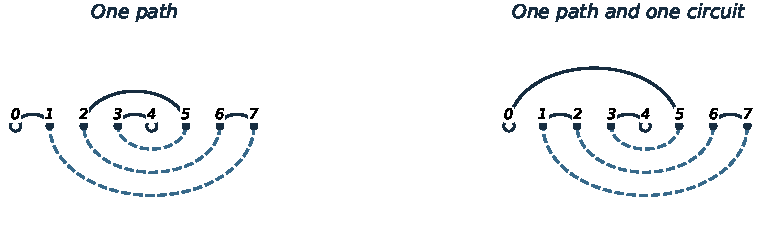
\includegraphics[width=.81\linewidth]{symmetric_example.pdf}
\caption{The two-end test on eight labels. The dashed reflection edges leave sites 0 and 4 exposed (open circles). There are ten choices of upper matching leading to one path. They give \(K_3=5\) shapes.}
\end{figure}
\section{A transfer with two marked ends}
\label{sec:axis-transfer}

Place the labels \(0,\ldots,2n-1\) around a circle. Draw a noncrossing
perfect matching \(A\) in the disk. Outside the disk join \(i\) to
\(-i\bmod 2n\), leaving \(0\) and \(n\) unmatched. The union consists of a
path between these two labels and a collection of cycles. Write
\(D(n,h)\) for the number of matchings for which the path uses every vertex
and exactly \(h\) chords of \(A\) join the two halves of the circle. Thus
\(0\le h\le n\), \(h\equiv n\bmod 2\), and \(D_n=\sum_h D(n,h)\).
All labels are retained in this count.

Write \(L_i=i\) and \(R_i=2n-1-i\), for \(0\le i<n\). Read each sequence
in increasing order of its subscript. Reading a half gives a ballot path.
An opening adds a vertex to a stack. A closing joins the new vertex to
the top of the stack and removes that entry. The two terminal heights are
both \(h\). The remaining vertices of equal rank from the bottom of the
two stacks must be joined because exchanging two partners introduces a crossing.
Conversely, two ballot paths of length \(n\) ending at \(h\), with this
last joining rule, determine one noncrossing matching. This gives the
orders of the two stacks as well as the multiplicity of every history.

Read \(L_0\) first, then the pairs \((L_t,R_{t-1})\) for \(1\le t<n\),
and finally \(R_{n-1}\). Each pair in this list is an exterior edge.
After the first vertex has been read there is exactly one exposed port
on the path from \(0\). Call it the marked port. Each other path in the
partial graph pairs two ordinary ports. A cycle at any intermediate
stage is disjoint from the final path and can be discarded. Around the
cut the ports occur in the order
\[
  (\text{left stack from bottom to top},\quad
   \text{right stack from top to bottom}).
\]
Deleting the marked port leaves a noncrossing pairing since the paths are
disjoint in the explored disk. Hence a balanced parenthesis word records
the ordinary pairs. The transfer stores its bits, the position of the
marked port, the length, the division between the stacks, and the
remaining target height.

An opening on both sides inserts an adjacent matched pair at the division
between the stacks. If one vertex opens and the other closes, the closing
port is extended to the new opening. The cyclic word stays the same and
the division moves by one position. Two closings join the adjacent ports
on either side of the division. Joining the two ends of the same path
would create a cycle. Otherwise their former partners become a pair, or
the partner of an ordinary port becomes marked if the other port was
marked. Joining the first and last ports obeys exactly the same rule,
since those two positions are adjacent on the circle.

\paragraph{Forced pairs.}
Suppose that \(a\) unread vertices remain on the left and \(a+1\) on the
right. Let \(u,v\) be the retained stack heights and \(r\) the common
terminal height after previous forced joins have been removed. A
continuation requires \(|u-r|\le a\) and \(|v-r|\le a+1\), with the
appropriate parities. The left path has precisely \((a+u-r)/2\)
closings still to come. Even if all of them remove existing vertices,
the bottom \((u+r-a)/2\) vertices will survive whenever this number
is positive. The corresponding statement on the right shows that
\[
 q=\max\left\{0,\min\left(\frac{u+r-a}{2},
                             \frac{v+r-a-1}{2}\right)\right\}
\]
bottom pairs can be joined immediately. Remove the corresponding bottom
port from each stack and decrease \(r\) once per pair. All these edges
belong to every completion and have the stated partners because previous
joins removed an equal number of bottom ports on both sides. Adding an
edge early preserves its contribution to connectivity. This is the
two-end form of the forced-bottom-pair rule of Zhang and Ma
\cite{zhangma2026}.

The retained cut has at most \(2j+1\) ports for
\(j=(n-h)/2\), uniformly in \(n\). Indeed, let \(x,y\) count closings
already used on the left and right. Removing the same number of ports
from both stacks preserves \(u-v=1+2(y-x)\). Once all forced pairs have
been removed, either \(u\le j-x\) or \(v\le j-y\). Otherwise another
bottom pair would survive both stacks. In the first case
\(u+v=2u-(u-v)\le2j-2y-1\), and in the second
\(u+v=2v+(u-v)\le2j-2x+1\).

After the final paired step, feasibility gives \(u=r\) and
\(v\in\{r-1,r+1\}\). Applying the forced joins leaves a single marked
port. If \(v=r+1\), this port is on the right and \(R_{n-1}=n\) closes
it. If \(v=r-1\), the port is on the left and \(R_{n-1}\) opens on the
right and is its forced cross-half partner. Thus each surviving history
has one final move. The initial history for \(n=1\) also gives one
matching. At every earlier layer, histories with the same state have
identical continuations and their integer weights add. This proves that
the output of a height sector is \(D(n,h)\).

There is also a bound on intermediate integer weights. At a fixed
layer and height, each retained pair of ballot prefixes extends to a
pair of complete paths of height \(h\) if connectivity is temporarily
ignored. The parity and distance tests are precisely the conditions for
such an extension. Different prefixes remain distinct after extension.
Consequently even the sum of the weights at that layer is at most
\(\bigl(\binom{n}{j}-\binom{n}{j-1}\bigr)^2\), where
\(j=(n-h)/2\) and \(\binom{n}{-1}=0\). It is also at most the Catalan
number \(C_n\), by the bijection with disk matchings. The wide version
checks its additions and imposes \(n\le61\), for which \(C_{61}<2^{128}\).
There is also a sector-dependent 64-bit limit on the packed state key.
All heights fit through \(n=46\). At \(n=47,h=1\) the present layout
requires 66 bits. The version with 64-bit weights checks each addition.

\begin{proposition}[Reading earlier orders from two states]
\label{prop:earlier-orders}
Run the sector with terminal order \(N\) and height \(H=N-2j\). At its
layer \(t\), after the first vertex and \(t\) paired steps, put
\(a=N-1-t\). For \(m=t+1\ge2j\), the number \(D(m,m-2j)\) is the sum
of the weights of two states. One has a single marked left port with remaining
target \(r=a+1\). The other has a single marked right port with \(r=a\).
An absent state contributes zero. Consequently all the sectors at
order \(N\) determine the complete triangle through order \(N\) with
no additional weighted transitions.
\end{proposition}

\begin{proof}
Fix \(j\). The raw numbers of remaining closings after \(x,y\) have
already occurred are \(j-x,j-y\), independent of \(N\). The same
bottom ranks are consequently forced for every choice of terminal
order on this diagonal. A history ending at the smaller order can
be prolonged to the larger cut by inserting as many double openings as
necessary before reading its last marked vertex. From either surviving
one-port state, such a step inserts a matched adjacent pair and then
joins the marked port to one of its ends. It leaves a single marked
port on the same side and consumes no closing. Thus the larger horizon
does not prune a history that contributes at the smaller one.

Let \(k=H-r\) bottom pairs have been removed. At layer \(t\) the
retained heights are \(u=t+1-2x-k\), \(v=t-2y-k\). At the smaller
order the left half is complete, so \(x=j\). When \(y=j\), the terminal
right vertex opens and the surviving left port gives
\(k=t-2j\), hence \(r=N-t=a+1\). When \(y=j-1\), it closes and the
surviving right port gives \(k=t+1-2j\), hence \(r=N-1-t=a\).
Conversely those one-port states give exactly these closing counts
and admit the indicated last move. Reading their two weights therefore
counts exactly the smaller sector.
\end{proof}

\begin{proposition}[Extending a stored layer]\label{prop:lift-layer}
Fix \(j\ge0\), orders \(N>N_0\ge\max(1,2j)\), and a cut
\(0\le t<N_0\). Put \(B=N_0-j\). Every state of the layer at \(N_0\)
occurs with its original weight at \(N\) after increasing the residual
target \(r\) by \(N-N_0\). The complementary states are precisely those
with \(x\le t-B\) or \(y\le t-B-1\), where \(x,y\) are the left
and right closing counts. To compute the complement, at each cut
\(0\le s\le t\) keep only histories whose closing counts satisfy
\(x_s\le t-B\) or \(y_s\le t-B-1\). Both thresholds use the target
cut \(t\).
\end{proposition}

\begin{proof}
Each half has exactly \(j\) closings at either horizon. A prefix below
these closing budgets fits the shorter horizon exactly when its opening
counts do not exceed \(B\) on either side. At the given cut these
counts are \(t+1-x,t-y\). Opening counts are nondecreasing, so a
prefix satisfying both shorter budgets has respected them at every
earlier cut. Increasing the horizon adds the same constant to the
residual target and to the remaining length. This leaves both terms in
the forced-pair minimum unchanged. The shorter histories therefore
have the same pairing, stack division, marked end and weight after
relabeling the residual target. The remaining histories violate one
of the two opening budgets, giving the claimed bounds on \(x,y\).
Closing counts also increase monotonically, so one may discard a
history as soon as both closing bounds fail. Finally, the retained
state determines \(x,y\) through the two identities in the preceding
proof. The two parts consequently have disjoint sets of state keys.
\end{proof}

At \(N=46,H=10,t=28\), the layer retained from \(N_0=45,H_0=9\)
contributed 680\,309\,616 weighted states. The complement, given by
\(x\le1\) or \(y=0\), contributed 167\,252\,355 more. The two streams
were merged into a layer of 847\,561\,971 states. Generating the
complement took 881\,278\,232 candidate moves. A fresh larger-horizon
prefix must attempt at least the 4\,590\,120\,086 moves of the shorter
prefix because its source states embed at every earlier cut, with the same
available local moves before pruning. With the shorter layer already
available, the lift saved at least 80.8 percent of the candidate moves
up to this cut, in addition to requiring a linear pass over the two
input files. A separate finite comparison matched every key and weight
on 141 small layers against the independently built larger horizon.
Inverting the large merge also reproduced both original byte streams,
including their SHA-256 digests.

\paragraph{Streaming a layer.}
Partition a layer by \(b=u-v\). A paired step changes \(b\) by
\(-2\), \(0\), or \(2\). Each forced join leaves \(b\) unchanged. Read the
source groups in increasing order of \(b\). Immediately after processing
source group \(b\), every contribution to target group \(b-2\) has
arrived. The group may be written out and its table freed. At most
three target groups are resident, and each source state is read only
once. The number of weighted updates is exactly the same as in the
in-memory computation. Each saved layer records its state count and
a checksum of its keys and weights. The preceding layer is retained
until the complete successor has been installed as a restart point.

One can also keep a single target group by opening three sequential
cursors on the same source file. For target \(b\), read the source
groups \(b-2,b,b+2\) from the three cursors and apply only moves with
the required change in \(b\). Every candidate move has one prescribed
target group, so it is evaluated once. This version reads each source
record three times. Its largest hash table holds a single group.
For several of the largest sectors, complete binary layers were
written in lossless Zstandard blocks. Each cursor decodes the same
logical stream of keys and integer weights. Ordinary uncompressed
checkpoints can be used as inputs to this version. In a cross-check
at \(n=32,h=8\), the decoded intermediate files agreed byte for byte
with the ordinary version.

\paragraph{A check without prescribing the height.}
One may instead allow all common terminal heights in a single transfer.
The feasibility test becomes \(|u-v|\le2a+1\), and the number of
immediate joins that does not require knowing the terminal height is
\(\max\{0,\min(u-a,v-a-1)\}\). On the final cut the heights must differ by
one. Pair the common bottom ranks and join the unmatched top on the taller side
to \(n\) by a closing or by a new cross-half chord. The result
is accepted exactly when this leaves the single marked path. This
calculation checks the summation over sectors while sharing the local
pairing operations of the sector transfer.

There is an external control for every even \(n=2k\). At height zero
the two halves carry independent noncrossing perfect matchings on \(2k\)
vertices. Add the edge joining the marked ends so that the path becomes
a cycle. The exterior edges now identify \(L_i\) with \(R_{i-1\bmod n}\).
A cyclic shift of the right labels preserves its set of noncrossing
matchings. After the identifications, connectivity is therefore the
ordinary one-cycle test on two matchings of \(2k\) labels. This proves
\(D(2k,0)=M_k\).

\section{The fixed-deficit diagonals}
\label{sec:axis-diagonals}

For \(j\ge0\), set \(f_j(n)=D(n,n-2j)\) for \(n\ge\max(1,2j)\) and
zero for smaller \(n\). Let \(\Phi_m\) denote the \(m\)-th cyclotomic
polynomial and put
\[
 F_j(z)=\sum_{n\ge0}f_j(n)z^n,\qquad
 Q_j(z)=(1-z)^{2j+1}\prod_{k=1}^j\Phi_{2k+1}(z)^{j+1-k}.
\]

\begin{theorem}\label{thm:marked-diagonals}
The product \(Q_j F_j\) belongs to \(\mathbb{Z}[z]\) and has
degree at most \(\deg Q_j+4j+1\). The function \(f_j(n)\) is eventually
a quasipolynomial of degree \(2j\), of period dividing
\(\operatorname{lcm}(1,3,\ldots,2j+1)\). Its leading coefficient is
positive and rational. For \(j\ge1\) the coefficients of
\(n^{2j},n^{2j-1},\ldots,n^j\) are the same on all residue classes.
\end{theorem}

\begin{proof}
There are exactly \(j\) internal chords on each side. In the two half
words, distinguish the two endpoints of an internal chord from a through
endpoint. A through endpoint can occur only when the local stack of
internal chords is empty. Record unmatched through endpoints in a queue,
in the order in which they appeared. All entries belong to the same side.
An arriving through endpoint on the other side meets the first member
of this queue. This is forced by the order of cross-half partners.
Together with the two local stacks, the number of internal chords
opened on each side, the pairing of path ports, and the position of the
marked port, this determines all subsequent moves. The construction uses
the ordered queue familiar from Ferudun's fixed-deficit transfer for
ordinary semi-meanders \cite{ferudun2026}. Here the unmatched initial
vertex changes the parity of every free rotation.

For a direct numerical implementation, place the waiting queue below the
local stack on its own side. In the same cyclic port order as above, its
first member is then the first port on the left or the last port on the
right. A local closing consumes a port at the division between the stacks.
A through endpoint meeting the opposite queue consumes its oldest port.
These are different histories from the ballot-prefix transfer, since the
status of a through endpoint is decided when it arrives. If \(m\) is the
number of ports, \(s\) the number on the left, and \(e\) the signed queue
length (positive on the left), the number of right internal openings minus
the number of left internal openings is \((m-1)/2-s+e\). This follows by
subtracting the numbers of processed through vertices on the two sides.
Thus it is enough to store one opening count alongside the two stack
boundaries and the path data. The numerical check regenerates the
component labels on every move and verifies the nesting of the result.

Fix the types of the initial and final vertices. Delete all paired
steps at which both vertices are through endpoints. What remains is a
word of \(s\le4j\) paired steps, each containing at least one endpoint
of an internal chord. Between consecutive retained steps, and at the
two ends of this word, both-through steps are possible only if both
local stacks are empty. Suppose \(x,y\) internal chords have been
completed at such a gap on the left and right, respectively. The left
side has processed one more vertex than the right side. Thus its number
of processed through endpoints minus the corresponding number on the
right is
\[
                 d=1+2(y-x).
\]
In particular the queue has nonzero length \(|d|\). A both-through step
pairs the other side's new vertex with the head of the queue. Their
exterior edge extends this port to the new tail on the waiting side.
The effect on the ordered path data is a cyclic shift on \(|d|\) ports,
including the marked port. It creates no cycle. Hence the result of a
run depends only on its length modulo \(|d|\).

Fix the residues of the lengths in all such gaps. The intervening
transitions determine whether this entire choice is accepted. An
accepted choice contributes
\[
 z^{\,1+s+\sum_i r_i}\prod_i(1-z^{|d_i|})^{-1},
                 \qquad 0\le r_i<|d_i|.
\]
There are finitely many retained words and residue choices. Gaps at
which a stack is nonempty have length zero and contribute no factor.
At the other gaps the successive points \((x,y)\) lie on a monotone
unit-step lattice path from \((0,0)\) to \((j,j)\). Between distinct
such gaps at least one internal chord has been completed. Simultaneous
completions on the two sides may be ordered either way when drawing
the lattice path. Thus there are at most \(2j+1\) factors of \(1-z\).
For \(m=2k+1>1\), a denominator contributes \(\Phi_m\) precisely when
\(y-x\equiv k\bmod m\). The first and last visits to this residue each
lie at distance at least \(k\) from their respective ends of the path.
Consecutive visits are at least two steps apart. There are therefore
at most \(1+(2j-2k)/2=j+1-k\) visits if \(k\le j\), and none otherwise.
Every term has denominator dividing \(Q_j\), up to sign. On bringing a
term to that common denominator its numerator has degree at most
\[
 1+s+\sum_i (|d_i|-1)+\deg Q_j-\sum_i|d_i|
 \ \le\ \deg Q_j+4j+1 .
\]
This proves the polynomial assertion, including integrality.

Partial fractions at the roots of unity of the indicated orders
give the eventual quasipolynomial. The pole at \(1\) has order at most
\(2j+1\) and every other pole has order at most \(j\). It remains to
show that the exponent \(2j\) occurs. Choose well-separated starting
indices \(a_1<b_1<\cdots<a_j<b_j\), put a left adjacent chord at each
\(a_i\) and a right adjacent chord at each \(b_i\), and join the remaining
through endpoints in order. For one such block \(a<b\), contracting the
exterior edges takes \(L_i\) to \(v_i\) and \(R_i\) to \(v_{i+1}\).
The through chords in the shifted interval join \(v_i\) to \(v_{i-1}\)
for \(a+2\le i\le b+1\), and the two adjacent chords fill its end edges.
Outside this block \(v_i\) is joined to \(v_{i+1}\). Several disjoint
blocks give the same path in succession. Choosing each of the \(2j\)
indices in its own interval of length proportional to \(n\) supplies
\(\Omega(n^{2j})\) distinct accepted configurations. The pole at \(1\)
must consequently have order \(2j+1\), and its leading coefficient is
positive. Its principal part has rational coefficients, while the other
poles contribute only through degree \(j-1\). For \(j=0\) the unique
all-through diagram gives \(F_0=z/(1-z)\).
\end{proof}

\paragraph{The first nonconstant diagonal.}
For \(j=1\) the sole internal chords start at indices \(a,b\) with
\(0\le a,b\le n-2\). The preceding path argument also covers \(a=b\),
when the shifted interval is empty. For \(a>b\) write \(d=a-b\).
After contracting the exterior edges, subtract \(b\) from vertex indices
in the active interval. The edges there are
\((i,i+3)\), \(0\le i<d\), together with \((1,2)\) and \((d,d+1)\).
The step-three edges form three chains, one in each residue class
modulo \(3\), allowing isolated vertices as chains of length zero.
The two short edges create a separate cycle exactly when they join
the same two classes, that is, when \(d\equiv1\bmod3\). Hence for \(n\ge2\)
\[
        D(n,n-2)=(n-1)^2-\sum_{k\ge0}\max(0,n-2-3k).
\]
Equivalently,
\[
        F_1(z)=\frac{z^2(1+z+2z^2+z^3)}
                         {(1-z)^3(1+z+z^2)}.
\]

\paragraph{Computed diagonal functions.}
The queue transfer gives the first \(\deg Q_j+4j+2\) coefficients,
including the constant term, with integer arithmetic. By the theorem
these determine the complete numerator of \(F_j\) with denominator
\(Q_j\). For \(0\le j\le7\), polynomial division gives
\(\gcd(Q_j,Q_jF_j)=1\) in every case. Thus all the stated cyclotomic
multiplicities, and the corresponding periods, are attained in this
range. The coefficient of \(n^{2j}\) is
\[
 \frac{(Q_jF_j)(1)}
 {(2j)!\prod_{k=1}^j\Phi_{2k+1}(1)^{j+1-k}}.
\]
For \(j=1,2,3,4\) its values are respectively \(5/6\), \(35/216\),
\(46367/3402000\), and \(12702127/20003760000\).
\begin{center}
\small\setlength{\tabcolsep}{3pt}
\begin{tabular}{r|rrrrrrrr}
\(j\) & 0&1&2&3&4&5&6&7\\
\hline
\(\deg Q_j\) &1&5&13&27&47&77&119&169\\
minimal period &1&3&15&105&315&3465&45045&45045\\
peak layer size &1&13&96&552&2807&13303&60432&267175
\end{tabular}
\end{center}

\paragraph{A smaller transfer for the leading coefficient.}
It is possible to compute the coefficient \(c_j\) of \(n^{2j}\) without
forming \(F_j\). Keep only the retained words in the proof that have
\(2j+1\) free gaps. Between successive gaps precisely one internal
chord must open and close. Its endpoints are consecutive on its side,
and both vertices on the opposite side are through endpoints. A local
chord using the initial or final marked vertex removes a free gap.
Two overlapping local chords also reduce the number of free gaps. Such
histories contribute poles of order at most \(2j\). The full-order
histories are consequently indexed by a shuffle of \(j\) left and
\(j\) right adjacent chords, together with the lengths of the gaps.

At a free gap identify cyclic port orders up to rotation, anchoring the
unique marked port at position zero. For a shuffle prefix with \(x\)
left and \(y\) right chords put \(d=1+2(y-x)\). Define
\(T_{d,d'}\), where \(d'=d\pm2\), on the marked noncrossing pairings of
\(|d|\) ports. If \(|d'|>|d|\), insert an adjacent matched pair in
each of the \(|d|\) gaps of the cyclic order, with weight \(1/|d|\)
per gap. If \(|d'|<|d|\), join each of the \(|d|\) adjacent pairs in
turn with the same weight, discarding any choice that closes a cycle.
If \(|d'|=|d|\), then \(|d|=1\) and the single marked port passes to
the other side. These rules follow by reading the two vertices of the
new local chord. The opposite through endpoints either extend the
waiting queue by a matched pair or consume its first two entries.

Start with unit mass \(v_{0,0}\) on the single marked port. From
\((x,y)\), add \(T_{d,d-2}v_{x,y}\) to \(v_{x+1,y}\) when \(x<j\),
and \(T_{d,d+2}v_{x,y}\) to \(v_{x,y+1}\) when \(y<j\). Then
\[
                       c_j=\frac{\|v_{j,j}\|_1}{(2j)!}.
\]
Indeed, each fixed residue at a free gap contributes
\(\lim_{z\to1}(1-z)/(1-z^{|d|})=1/|d|\) to the leading pole.
Summing over all residues gives precisely the averaged operation
\(T_{d,d'}\), and the last queue has length one. The factor \((2j)!\)
converts the principal part to a leading coefficient. This supplies
an independent evaluation of the seven nonconstant leading
coefficients above. For example the next value is
\[
c_8=\frac{512292467507145510289931917}
          {7983707178219937782841903680000000000}.
\]

\paragraph{Comparison with the rainbow.}
For ordinary semi-meanders the fixed exterior matching is
\(i\mapsto2n-1-i\). It pairs \(L_t\) with \(R_t\) and has no marked
ends. Zhang and Ma prove eventual degree \(2j-2\) and a period dividing
\(2\operatorname{lcm}(1,\ldots,j)\) for that model, and give rational
certificates for its third and fourth diagonals \cite{zhangma2026}.
Their paired readings, immediate bottom joins and rotation of the
surviving ports underlie the comparison. In the present model the
readings differ by one vertex. The discrepancy \(1+2(y-x)\) at an
empty-stack gap is always odd, including at the initial and final
levels. These extra possible rotations account for the change in
degree, and the lattice path bounds each odd cyclotomic multiplicity
separately. At height \(h=n\) the marked
model has a path for every \(n\), whereas the ordinary rainbow has
\(n\) two-edge components.


\section{Values and external comparisons}
The public OEIS file for A223096 ends at \(K_{22}=9\,962\,795\,554\) \cite{sseq}. The wheel of \textit{mapFolding} 0.40.1, released on 17 November 2026, contains nine further terms through \(K_{31}\). The public repository on the same date adds \(K_{32}=1\,650\,268\,613\,634\,453\) \cite{hogan}. The disk calculation agrees through \(K_{27}\). Two earlier implementations of the reflected transfer agree through \(K_{30}\). The marked-path transfer gives all the values listed below, including those for which an external value exists.

\begin{table}[htbp]\centering
\begin{tabular}{rr@{\hspace{2em}}rr}\toprule
Index&\(K_k\)&Index&\(K_k\)\\\midrule
23 & 32\,846\,647\,658 & 35 & 62\,567\,332\,433\,552\,830\\
24 & 108\,498\,959\,945 & 36 & 210\,636\,220\,209\,732\,928\\
25 & 359\,367\,363\,740 & 37 & 709\,999\,304\,027\,656\,342\\
26 & 1\,192\,228\,650\,177 & 38 & 2\,395\,099\,469\,566\,939\,312\\
27 & 3\,964\,528\,526\,244 & 39 & 8\,088\,627\,634\,690\,725\,560\\
28 & 13\,201\,939\,675\,885 & 40 & 27\,335\,977\,176\,330\,801\,104\\
29 & 44\,051\,514\,192\,054 & 41 & 92\,477\,031\,405\,925\,909\,792\\
30 & 147\,170\,887\,842\,404 & 42 & 313\,050\,008\,470\,252\,133\,808\\
31 & 492\,550\,457\,391\,043 & 43 & 1\,060\,701\,561\,590\,886\,000\,892\\
32 & 1\,650\,268\,613\,634\,453 & 44 & 3\,596\,076\,920\,714\,729\,163\,608\\
33 & 5\,537\,787\,877\,254\,848 & 45 & 12\,201\,962\,983\,536\,099\,355\,104\\
34 & 18\,601\,185\,486\,419\,129 &  & \\
\bottomrule\end{tabular}
\caption{Symmetric open shapes by index. Index \(k\) corresponds to \(2k+1\) physical crossings.}
\end{table}
At index 45 the full sector sum accounts for 144\,193\,608\,212 attempted moves. The largest individual process recorded for the selected runs used 3.21 GiB. The fixed-deficit queue calculation independently checks the outer seven sectors of each extension. At an even disk order the zero-height sector equals the ordinary closed count at half that order. A computation with an unspecified final height independently reproduced the marked-path totals through disk order 34. At shape index 33, the first past the public table, an independent queue transfer agreed in every height sector. The attached records distinguish these partial checks from agreement of two full enumerations.

For a separate timing experiment we compiled Hogan's published \texttt{cpp-pile} counter and the marked-path program with the same optimization settings and pinned them to one CPU on the same machine. Each call computed the whole shape count. With four tail layers and an equal 730 MiB memory limit at \(k=26\), the two runs took 80.59 and 75.48 seconds for Hogan's program and 1.222 and 1.205 seconds for the marked-path calculation. All four returned \(1\,192\,228\,650\,177\). The ratio of the two medians was 64.3. At \(k=24\) the observed median ratio at four tail layers was 32.9; the supplement also records results with the tail depth varied. These timings concern the named implementations and input orders. Each timing file records parameters, run order, and memory limits. Other local calculations shared the host.

\section{All open shapes at odd lengths}
Write \(a(\ell)\) for all open meander shapes at length \(\ell\), including asymmetric shapes. Legendre's formulas read
\[
 a(2p+1)=\frac{M_{p+1}+2K_p}{4},\qquad
 a(2p)=\frac{m(2p)+m(p)}{2}\qquad(p\ge1).
\]
The archived ordinary closed count runs through \(M_{38}\). The new symmetric data therefore give each odd value through \(a(75)\), with \(a(1)=1\). The labelled open even sequence supplies all even values through 58. Representative values are
\begin{center}
\begin{tabular}{rr}\toprule
Crossings \(\ell\)&All shapes \(a(\ell)\)\\\midrule
59 & 319\,960\,722\,152\,016\,248\,206\,479\,788\\
65 & 428\,415\,405\,209\,401\,772\,951\,427\,083\,588\\
67 & 4\,751\,908\,454\,324\,444\,995\,437\,008\,580\,879\\
71 & 589\,565\,459\,687\,932\,286\,086\,752\,243\,007\,918\\
75 & 73\,899\,520\,455\,701\,062\,036\,121\,592\,186\,576\,909\\
\bottomrule\end{tabular}
\end{center}
At length 77 the symmetric summand is now known, while the other summand is the full integer \(M_{39}\). The congruence \(M_{39}\equiv16\bmod312\) from the companion paper on closed-count congruences gives \(a(77)\equiv60\bmod78\). The supplement tabulates the labelled count, symmetric correction and exact quotient at each available length. The official A077055 b-file retrieved in November started at index zero for physical length one. Hogan's additional table uses the physical length itself \cite{shapes,hogan}. Direct comparison uses the translated indices. The published symmetric terms through \(K_{32}\) already imply odd shape counts through length 65. The new symmetric inputs first enter at length 67.

\section*{Sources and reproduction}
The supplement records exact integers, sector totals, timing and memory for completed runs, and the numerator and denominator of the fixed-deficit functions. Its verifier checks the finite Catalan examples, the external terms, all available sector sums, and the reconstruction of the open shapes. It can replay complete indices or individual sectors. Comparisons with earlier publications concern the conventions and files specified above.
\begin{thebibliography}{9}\small
\bibitem{legendre} S.~Legendre, Foldings and meanders, \emph{Australas. J. Combin.} \textbf{58} (2014), 275--291. \href{https://ajc.maths.uq.edu.au/pdf/58/ajc_v58_p275.pdf}{Article}.
\bibitem{sseq} OEIS Foundation, \href{https://oeis.org/A223096}{A223096}, symmetric meander shapes at odd crossing counts.
\bibitem{hogan} H.~Hogan, \emph{mapFolding} \href{https://pypi.org/project/mapFolding/0.40.1/}{0.40.1}; \href{https://github.com/hunterhogan/mapFolding/blob/1862930c2f0bfe5a38ae8cd299e6b85eaa1dc632/mapFolding/oeis/terms/files/A223/b223096.txt}{symmetric counts through index 32}, 17 November 2026.
\bibitem{zhangma2026} W.~Zhang and H.~Ma, \emph{Semi-meanders with a fixed winding deficit: the third and fourth diagonals of A400429}, 6 October 2026. \href{https://oeis.org/A400429/a400429.pdf}{Manuscript}.
\bibitem{ferudun2026} A.~Ferudun, fixed-deficit semi-meander transfer, October 2026. \href{https://github.com/hunterhogan/mapFolding/blob/1862930c2f0bfe5a38ae8cd299e6b85eaa1dc632/research/matrixMeanders/fixed_deficit_semimeanders.py}{Source in mapFolding}.
\bibitem{dg} P.~Di Francesco, O.~Golinelli and E.~Guitter, Meanders: a direct enumeration approach, \emph{Nuclear Phys.~B} \textbf{482} (1996), 497--535. \href{https://arxiv.org/abs/hep-th/9607039}{Preprint}.
\bibitem{shapes} OEIS Foundation, \href{https://oeis.org/A077055}{A077055}, \href{https://oeis.org/A078592}{A078592}, \href{https://oeis.org/A005315}{A005315} and \href{https://oeis.org/A005316}{A005316}.
\end{thebibliography}
\end{document}
